\section{Feature Extraction and Feature Fusion}
\label{sec:FeatureExtractionFusion}

It goes without saying that efficient capabilities of deep learning models of extracting robust features pertinent to the task at hand are of great significance. As we have observed in our survey of Siamese trackers~\cite{ondrasovic2021siamese}, incremental improvements in feature extraction were often the major contribution of numerous works that granted the authors a competitive performance against other \gls{sota} frameworks. With this in mind, we consider feature extraction a necessary part of any deep learning model design. As we will see further, the model with which we performed majority of our experiments exploited top feature extraction approaches. Thus, it is also suitable to provide a brief background to the most influential methods of feature extraction and feature fusion. Overall, the later introduced \gls{fpn} as well as \gls{dla} approaches to feature fusion stand at the code of feature extraction when it comes to our further experiments.

% ##############################################################################
\subsection{Residual Neural Networks}
\label{ssec:ResidualNeuralNetworks}

He~\etal{}~\cite{he2015resnet} aptly remarked that deeper neural networks are more difficult to train. In their work, the authors proposed a residual learning framework to facilitate easier training of neural networks that were significantly deeper than their previously used counterparts. The explicit reformulation of the layers as learning residual functions with reference to the layer inputs, instead of learning unreferenced functions, led to a breakthrough in the harnessing of deep neural networks. The proposed architecture was dubbed as \gls{resnet}.

The foundation of \glspl{resnet} is the utilization of skip connections that represent shortcuts to jump over some layers. Typically, such models are implemented using double or even triple layer skips containing nonlinearities (e.g., \gls{relu}) and batch normalization~\cite{ioffe2015batchnorm} in between.

The primary reason for adding skip connections was to avoid vanishing gradient problems. As demonstrated in \figstr{}~\ref{fig:ResnetMotivation}, the degradation problem manifests itself out in deeper networks when their accuracy shows signs of saturation followed a by rapid decline, but not as a result of overfitting. By construction, a deeper network could at least learn an identity mapping, i.e., to copy the previous value, and thus yield at least the same performance, but not worse. This degradation problem can be effectively addressed using residual learning by additing the aforementioned skip connections.

Specifically, let $\func{H}{\vect{x}}$ denote the desired underlying mapping. The stacked nonlinear layers are then expected to fit a different mapping $\func{F}{\vect{x}} = \func{H}{\vect{x}} - \vect{x}$. Thus, the original mapping is reformulated as $\func{H}{\vect{x}} = \func{F}{\vect{x}} + \vect{x}$. The initial hypothesis, which turned out to be correct, was that it is easier to optimize the residual mapping instead of the original, unreferenced mapping. This formulation is visualized on \figstr{}~\ref{fig:SkipConnections}.

% ------------------------------------------------------------------------------
\begin{figure}[t]
    \centerline{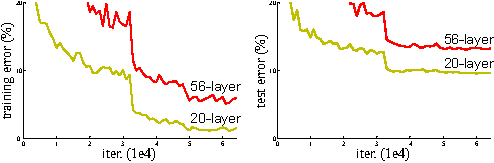
\includegraphics[width=0.9\linewidth]{figures/theoretical_foundations/resnet_motivation.pdf}}
    \caption[\Gls{resnet} motivation]{The motivating behind the introduction of \glspl{resnet}. The training error, and thus the test error as well, is greater for the deeper model than for the shallower model. Therefore, the inevitable conclusion is that in order to learn better networks, it takes more than just stacking more layers. \externalsrc{\cite{he2015resnet}}}
    \label{fig:ResnetMotivation}
\end{figure}

% ------------------------------------------------------------------------------
\begin{figure}[t]
    \centerline{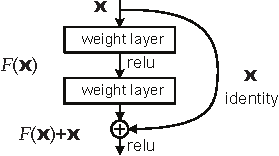
\includegraphics[width=0.35\linewidth]{figures/theoretical_foundations/skip_connections.pdf}}
    \caption[Skip connections]{A basic building block of residual learning demonstrating the mapping reformulation using skip connections. \externalsrc{\cite{he2015resnet}}}
    \label{fig:SkipConnections}
\end{figure}

To highglight the importance of these ideas, \Gls{resnet} was used as the foundational backbone architecture for feature extraction in majority of all our experiments.

% ##############################################################################
\subsection{Feature Pyramid Networks}
\label{ssec:FeaturePyramidNetworks}

When detecting objects visually at different image resolutions, pyramidal feature aggregation brings significant improvements at negligible computational overhead. \Gls{fpn}~\cite{lin2017fpn} is an extension to existing backbones used for feature extraction serving various tasks ranging from image classification, object detection, object tracking or even image segmentation. Its greatest strength is the combination of low-resolution, semantically strong features with high-resolution, semantically weak but discriminative features via a top-down pathway and lateral connections.

\figstr{}~\ref{fig:FPNVariousApproaches} compares competing methods of feature aggregation by their core principles. Regarding the \gls{fpn} itself, observe the two pathways in \figstr{}~\ref{fig:FPNVariousApproaches} \imgpartdesc{d}. The bottom-up pathway represents a feedforward computation of the backbone (e.g., a basic \gls{cnn}), where one pyramid levels corresponds to one stage. The output of the last layer of each stage will serve the purpose of enriching the feature maps when processing the top-down pathway by use of lateral connections. The top-down pathway consists of upsampling operations followed by an application of $1 \times 1$ convolutions to align tensor channels dimensions and then element-wise addition of features. Each lateral connection merges features of the same spatial size at each stage from the two pathways. If applied to a model, a rich feature representation is then available for further processing, e.g., detecting objects, thus greatly enhancing the model performance.

% ------------------------------------------------------------------------------
\begin{figure}
    \centering
    \begin{subfigure}[t]{0.4\textwidth}
        \centering
        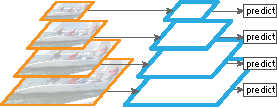
\includegraphics[width=\textwidth]{figures/theoretical_foundations/fpn_featurized_image_pyramid.pdf}
        \caption[]{}
    \end{subfigure}
    \hfill
    \begin{subfigure}[t]{0.4\textwidth}
        \centering
        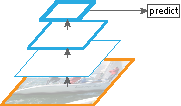
\includegraphics[width=\textwidth]{figures/theoretical_foundations/fpn_single_feature_map.pdf}
        \caption[]{}
    \end{subfigure}

    \begin{subfigure}[t]{0.4\textwidth}
        \centering
        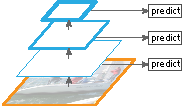
\includegraphics[width=\textwidth]{figures/theoretical_foundations/fpn_pyramidal_feature_hierarchy.pdf}
        \caption[]{}
    \end{subfigure}
    \hfill
    \begin{subfigure}[t]{0.4\textwidth}
        \centering
        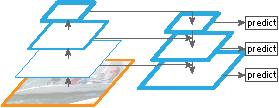
\includegraphics[width=\textwidth]{figures/theoretical_foundations/fpn_feature_pyramid_network.pdf}
        \caption[]{}
    \end{subfigure}
    \caption[\gls{fpn}]{A comparison of four traditional approaches to feature aggregation. \imgpartdesc{a} Computing features on distinct image scales (computationally expensive); \imgpartdesc{b} the use of single scale features only (fast, but not robust); \imgpartdesc{c} Reusing pyramidal feature hierarchy (fast and robust); \imgpartdesc{d} the proposed \gls{fpn} - pyramidal feature aggregation in both directions (practically fast as previous methods but considerably more accurate). \externalsrc{\cite{lin2017fpn}}}
    \label{fig:FPNVariousApproaches}
\end{figure}

% ##############################################################################
\subsection{Deep Layer Aggregation}
\label{ssec:DeepLayerAggregation}

% ------------------------------------------------------------------------------
\begin{figure}[t]
    \centerline{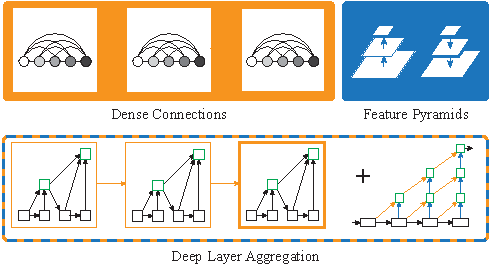
\includegraphics[width=0.7\linewidth]{figures/theoretical_foundations/dla_comparison.pdf}}
    \caption[\Gls{dla} comparison]{A demonstration of unification of semantic and spatial information. The \gls{dla} architecture extends densely connected networks, i.e., \glspl{densenet}, and \glspl{fpn}. This extension builds on the idea of skip connections for enhanced feature fusion. \externalsrc{\cite{yu2019dla}}}
    \label{fig:DLAMotivation}
\end{figure}

A successor of the previously discussed \gls{fpn} is the \gls{dla}~\cite{yu2019dla}. This architecture extension emphasizes the importance of feature aggregation across multiple levels in order to merge information from different stages of input processing (see \figstr{}~\ref{fig:DLAMotivation}). Experimentally, this technique shows significant improvements in both memory usage and performance over frequently employed baselines such as \gls{resnet}~\cite{he2015resnet} or \gls{densenet}~\cite{huang2018densenet}, to name a few. In contrast with the skip connections, the \gls{dla} introduces more depth and sharing. There are two main different approaches to \gls{dla}, namely \gls{ida} and \gls{hda} (see \figstr{}~\ref{fig:DLADiffApproaches} for further ideas). These structures are expressed through an architectural framework, which is, more importantly, independent of the choice of backbone, thus preserving the compatibility with current and future networks.

% ------------------------------------------------------------------------------
\begin{figure}[t]
    \centerline{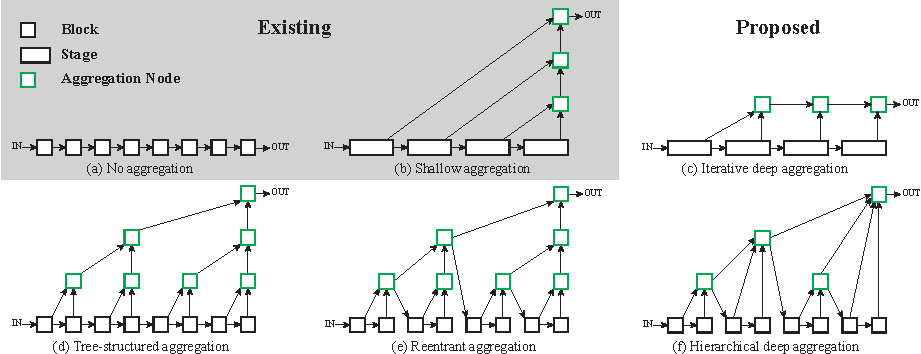
\includegraphics[width=0.8\linewidth]{figures/theoretical_foundations/dla_existing_vs_proposed.pdf}}
    \caption[\Gls{dla} proposed solution]{Different approaches to feature aggregation. \imgpartdesc{a} No aggregation; \imgpartdesc{b} Shallow aggregation using skip connections; \imgpartdesc{c} Reordering of skip connections; \imgpartdesc{d} shallowst parts are aggregated the most; \imgpartdesc{e}, \imgpartdesc{f} further refining for deeper aggregation by routing intermediate aggregations back into the network. \externalsrc{\cite{yu2019dla}}}
    \label{fig:DLADiffApproaches}
\end{figure}

\subsubsection{Iterative Deep Aggregation}

\gls{ida} aims at resolution and scale fusion. The process starts at the smallest scale and then iteratively merges larger (deeper) scales. This strategy can be mathematically described as
\begin{equation}
    \label{eq:IterativeDeepAggregation}
    \func{I}{\vect{x}_1, \vect{x}_2, \vect{x}_3, \dots, \vect{x}_n} =
    \begin{cases}
         & \vect{x}_1 \text{ if } n = 1                                                                \\
         & \func{I}{\func{A}{\vect{x}_1, \vect{x}_2}, \vect{x}_3, \dots, \vect{x}_n} \text{ otherwise}
    \end{cases},
\end{equation}
where $A$ is the aggregation node.

\subsubsection{Hierarchical Deep Aggregation}

\gls{hda} focuses on feature merging across all modules as well as channels. The process of aggregation exploits a tree-like structure to combine layers that span multiple levels of a feature hierarchy. The \gls{hda} with aggregation function $T_n$ with $n$ representing the depth can be formulated as
\begin{equation}
    \label{eq:HierarchicalDeepAggregation}
    \func{T_n}{\vect{x}} =
    \func{A}{
        \func{\subsup{R}{n - 1}{n}}{\vect{x}},
        \func{\subsup{R}{n - 2}{n}}{\vect{x}},
        \dots,
        \func{\subsup{R}{1}{n}}{\vect{x}},
        \func{\subsup{L}{1}{n}}{\vect{x}},
        \func{\subsup{L}{2}{n}}{\vect{x}}
    },
\end{equation}
where $A$ is the aggregation node as in \eqstr{}~\ref{eq:IterativeDeepAggregation}. The functions $R$ and $L$ are defined as follows
\begin{equation}
    \label{eq:HDAConvBlocksL}
    \begin{aligned}
         & \func{\subsup{L}{1}{n}}{\vect{x}} = \func{B}{\func{\subsup{R}{1}{n}}{\vect{x}}}, \\
         & \func{\subsup{L}{2}{n}}{\vect{x}} = \func{B}{\func{\subsup{L}{1}{n}}{\vect{x}}}
    \end{aligned}
\end{equation}
and
\begin{equation}
    \label{eq:DLAConvBlocksR}
    \func{\subsup{R}{m}{n}}{\vect{x}} =
    \begin{cases}
         & \func{T_m}{\vect{x}} \text{ if } $m = n - 1$                        \\
         & \func{T_m}{\func{\subsup{R}{m + 1}{n}}{\vect{x}}} \text{ otherwise}
    \end{cases},
\end{equation}
where $B$ represents some convolutional block.

\subsubsection{Combination of Both Approaches}

The two approaches above are independent as well as compatible enough to facilitate combining the two together for even richer feature aggregation as shown in \figstr{}~\ref{fig:DLACombination}.

% ------------------------------------------------------------------------------
\begin{figure}[t]
    \centerline{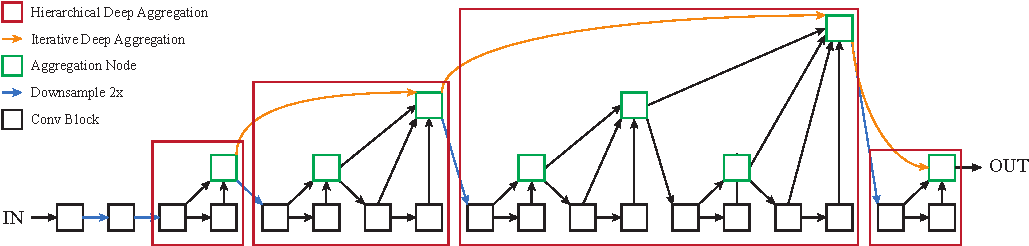
\includegraphics[width=0.9\linewidth]{figures/theoretical_foundations/dla_ida_hda_combination.pdf}}
    \caption[Combination of \gls{dla} approaches]{\Gls{dla} promotes enhanced feature extraction in spatial and semantic spectrum from the underlying network. In this combined approach, iterative connections progressively deepen and spatially refine the feature representation by joining neighboring stages. Simultaneously, hierarchical connections cross these stages with a tree-like structure to aid gradient propagation through the model. \externalsrc{\cite{yu2019dla}}}
    \label{fig:DLACombination}
\end{figure}
